\chapter[Marco Teórico]{Marco Teórico}
\label{cp:theoretical-framework}

\parindent0pt

% TODO: fix redaction of all sections, add references, and improve the connection between sections

Este capítulo presenta los fundamentos teóricos que sirven de base para este trabajo. Se aborda la estructura y funcionamiento de las cadenas de bloques, destacando sus características de descentralización, transparencia e inmutabilidad, así como los mecanismos de consenso que garantizan su seguridad y eficiencia. Además, se analiza el rol de los contratos inteligentes como herramientas para automatizar procesos y gestionar la lógica de negocio en entornos descentralizados. Asimismo, este capítulo explora los principios de la economía circular, enfatizando su enfoque regenerativo y su capacidad para transformar las cadenas de suministro hacia modelos más sostenibles. Se examinan las etapas del proceso de producción y reciclaje, con especial atención a la trazabilidad como habilitador para garantizar la transparencia y la eficiencia en una economía circular. Luego se incluye un análisis de la cadena de suministro del vidrio en el contexto mendocino, destacando su relevancia estratégica y los desafíos asociados a su implementación en un modelo circular. Finalmente, se explora el estado del arte de la tecnología \textit{blockchain} en la economía circular, identificando las tendencias actuales y las oportunidades de mejora en la trazabilidad y sostenibilidad de la cadena de suministro del vidrio.

\section{Blockchain}

Para comprender la necesidad e impacto de la tecnología blockchain, primero es necesario analizar la arquitectura predominante de Internet hasta la actualidad, basada tradicionalmente en un modelo centralizado cliente-servidor. En este esquema, los datos son almacenados en servidores administrados por proveedores, quienes actúan como intermediarios de confianza entre los clientes o usuarios. Aunque este modelo ha facilitado el intercambio de información a escala masiva, también ha generado problemas de confianza, seguridad y privacidad. La centralización implica que los usuarios ceden el control y gestión de sus datos a terceros, lo que puede derivar en una dependencia significativa de estas entidades para la integridad y disponibilidad de la información. Ejemplos de esto incluyen la exposición de datos personales privados en ciber-ataques, la interrupción de servicios por fallas en servidores centrales o la censura de contenido por decisiones unilaterales de las plataformas \cite{pending}.

Ante los desafíos de confianza e integridad en los sistemas centralizados, la tecnología blockchain surgió en 2008 como una solución disruptiva. Su primera aplicación fue como base del sistema de criptomonedas Bitcoin \cite{satoshi2008bitcoin}, pero rápidamente demostró potencial por fuera del ámbito financiero. En la actualidad, blockchain se considera una herramienta útil para resolver problemas de confianza, transparencia e inmutabilidad en la gestión de datos. Su diseño permite registrar información de forma distribuida, sin necesidad de proveedores centralizados, habilitando la interacción directa entre múltiples partes \cite{bulkowska2023implementation}.

\begin{figure}[!htpb]
    \centering
    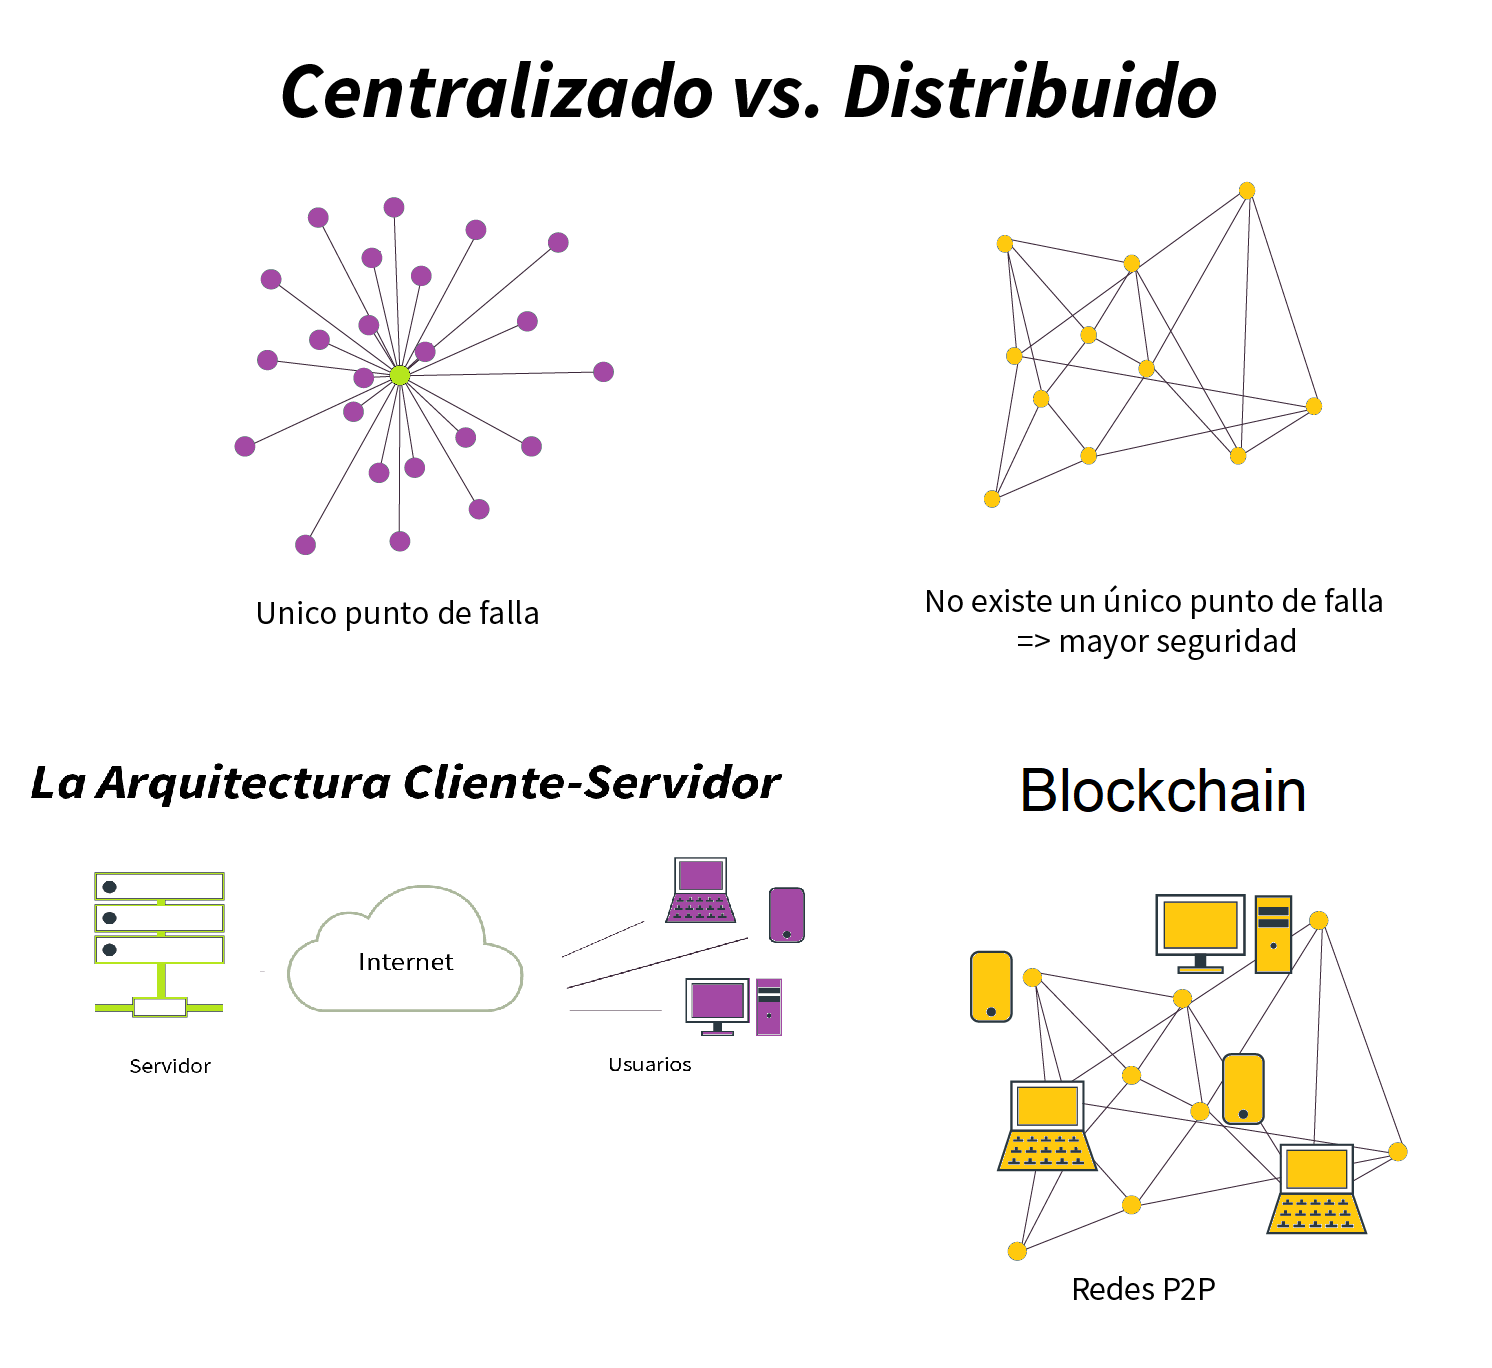
\includegraphics[width=0.8\textwidth]{Figures/cliente-server-vs-p2p.png}
    \caption{Comparación entre el modelo cliente-servidor y el modelo P2P}
    \label{fig:web-architecture}
\end{figure}

Es importante destacar que blockchain no introduce tecnologías completamente nuevas, sino que integra de forma innovadora principios existentes de la computación y las matemáticas. Combina conceptos de criptografía (para asegurar la información), redes distribuidas (para la replicación de los datos) y teoría de juegos e incentivos (para coordinar el comportamiento de los participantes y garantizar la seguridad de los datos) \cite{sunny2022systematic, bulkowska2023implementation}. Esta integración produce un sistema seguro, transparente y resistente a manipulaciones, características difíciles de lograr en modelos centralizados. De esta manera, blockchain impulsa un nuevo paradigma donde el registro de la información es gestionado colectivamente, lo que permite transacciones y acuerdos entre pares sin depender de un tercero de confianza.

\begin{figure}[!htpb]
    \centering
    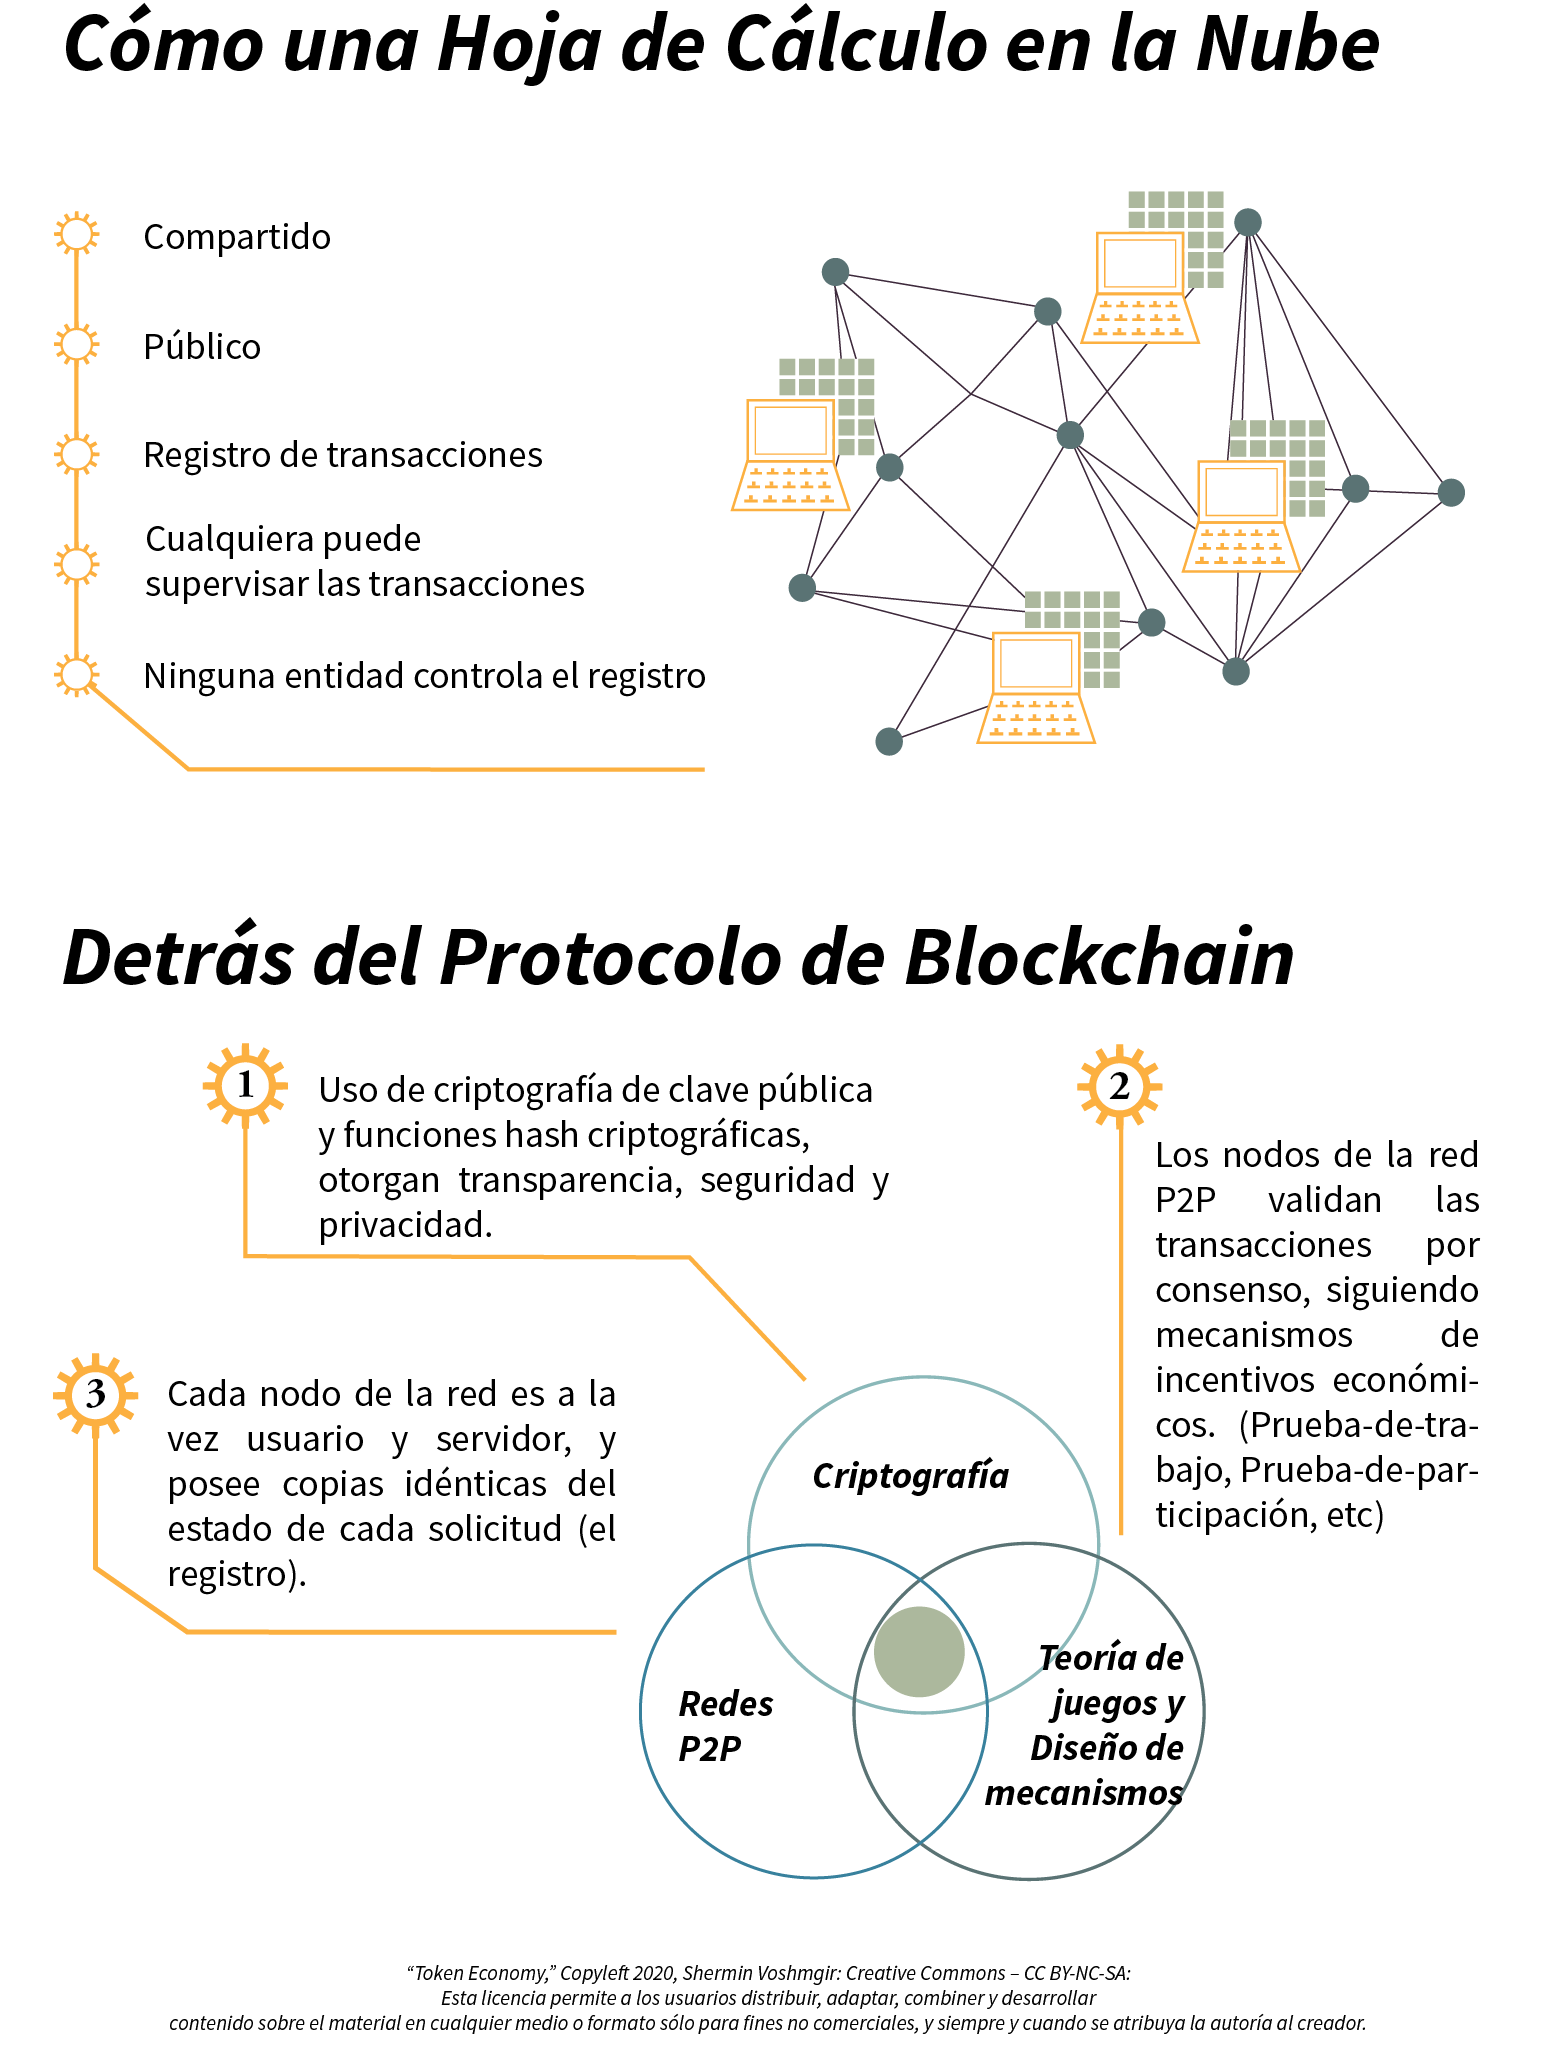
\includegraphics[width=0.8\textwidth]{Figures/venn-blockchain.png}
    \caption{Intersección de tecnologías y conceptos que componen la tecnología blockchain}
    \label{fig:blockchain-venn}
\end{figure}

En las próximas páginas se explorará en detalle la estructura y funcionamiento de la tecnología blockchain, sus características distintivas, los mecanismos de consenso que garantizan su seguridad y el papel de los contratos inteligentes como herramientas para la automatización de procesos. Además, se analizarán las ventajas y desafíos asociados a su implementación, así como su potencial de uso más allá del ámbito financiero.

\section{Estructura de una Blockchain}

La tecnología \textit{blockchain}, o cadena de bloques, es una estructura de datos distribuida y descentralizada donde la información se organiza en transacciones agrupadas en bloques enlazados criptográficamente. Cada bloque posee un código único, conocido como \textit{hash del bloque}, que lo identifica y sirve para enlazarlo al bloque posterior. El hash de cada bloque se genera a partir de su contenido y del hash del bloque anterior, creando así una cadena continua de bloques interconectados \cite{tripathi2023comprehensive}.

\begin{figure}[!htpb]
    \centering
    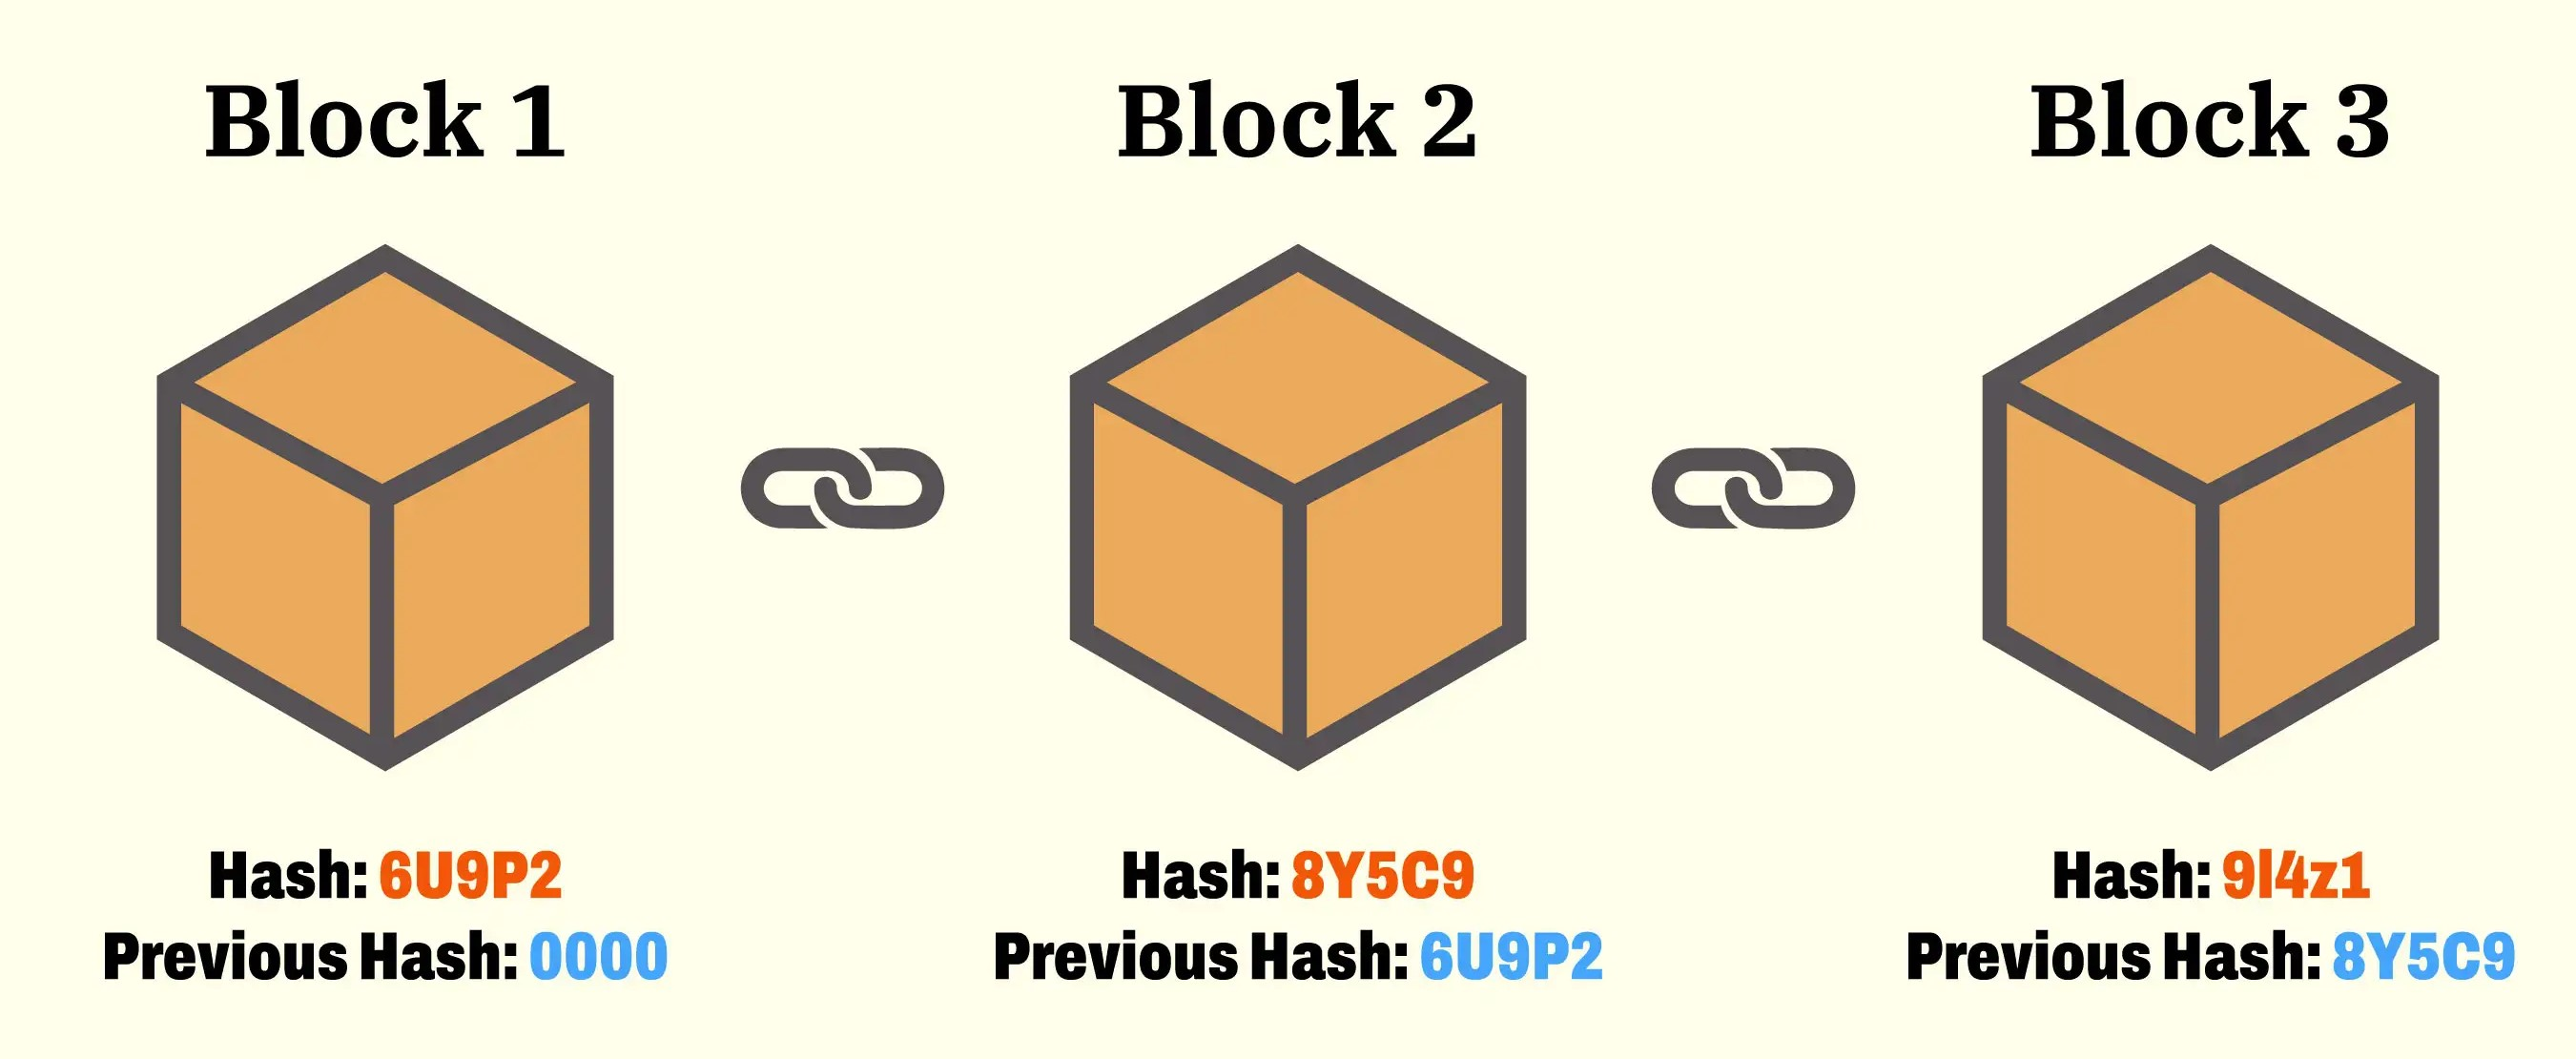
\includegraphics[width=0.8\textwidth]{Figures/blockchain-basic.jpg}
    \caption{Estructura básica de una cadena de bloques}
    \label{fig:blockchain-basic}
\end{figure}

Cada bloque de la cadena consta de un encabezado y un cuerpo \cite{tripathi2023comprehensive}. El cuerpo alberga la lista de transacciones, mientras que el encabezado contiene metadatos. Entre los metadatos se encuentran el código único del bloque anterior, una marca de tiempo, y el código que identifica unívocamente al bloque actual.

El código identificatorio del bloque, conocido también como \textit{hash del bloque}, se calcula mediante funciones hash criptográficas, que son algoritmos matemáticos que transforman datos de entrada en una cadena de caracteres de longitud fija. Los códigos hash tienen la propiedad de ser únicos para cada conjunto de datos, lo que significa que cualquier cambio en el contenido del bloque generará un código hash completamente diferente \cite{pending}. Esta característica permite verificar la integridad de los datos almacenados en la cadena, ya que el código hash de un bloque se puede recalcular en cualquier momento y comparar con el código almacenado en la cadena. Si los códigos coinciden, se puede confiar en que los datos no han sido alterados; si no coinciden, se ha producido una modificación no autorizada en el contenido del bloque \cite{pending}.

El encadenamiento criptográfico de bloques en una red descentralizada, como requiere la blockchain, garantiza la integridad e inmutabilidad de la información, ya que cualquier alteración en un bloque modificaría su hash y rompería la consistencia de la cadena, forzando a cada nodo de la red descentralizada a rechazar el bloque modificado o forzando a cada nodo a modificar los hashes de todos los bloques posteriores \cite{sunny2022systematic}. En la Figura \ref{fig:blockchain-structure} se ilustra la estructura de una blockchain, donde cada bloque contiene un hash del bloque anterior, formando una cadena de bloques interconectados criptográficamente.

\begin{figure}[!htpb]
    \centering
    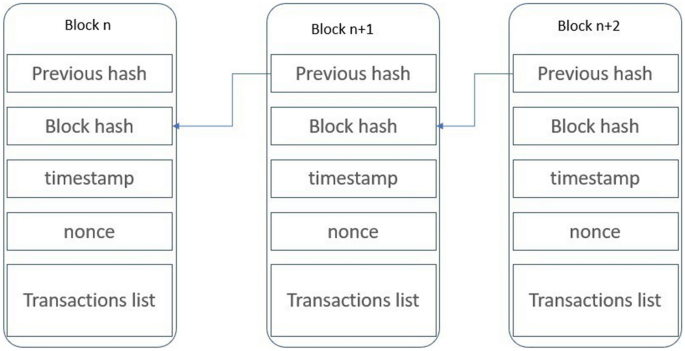
\includegraphics[width=0.8\textwidth]{Figures/blockchain-structure.png}
    \caption{Contenido de un bloque en una cadena de bloques}
    \label{fig:blockchain-structure}
\end{figure}


% Esta tecnología se caracteriza por algunas propiedades fundamentales: descentralización, transparencia e inmutabilidad. Estas propiedades la hacen especialmente adecuada para casos de uso que requieren confianza, seguridad y trazabilidad en la gestión de datos \cite{bulkowska2023implementation}.

% La tecnología blockchain fue implementada inicialmente en 2008 como el fundamento del sistema de criptomonedas Bitcoin \cite{satoshi2008bitcoin}. Desde entonces, ha trascendido el ámbito financiero para abarcar una amplia gama de aplicaciones \cite{bartolomeo2020introduccion}. Posteriormente, se han desarrollado diversos protocolos blockchain que han permitido la creación de redes más eficientes y adaptadas a distintas necesidades, como Ethereum \cite{buterin2013ethereum}, pionero en el concepto de contratos inteligentes, o Hyperledger \cite{androulaki2018hyperledger}, enfocado en aplicaciones empresariales \cite{sunny2022systematic, rennock2018blockchain}.


Su naturaleza distribuida radica en que cada nodo de la red mantiene una copia completa y actualizada del registro, lo cual asegura su transparencia y resiliencia al no depender de un servidor central \cite{bulkowska2023implementation}. Por su parte, la descentralización implica la ausencia de una autoridad central, ya que la validación y adición de nuevos bloques se rige por un mecanismo de consenso entre los nodos participantes de la red. 

La interconexión criptográfica entre los bloques confiere a blockchain su característica de inmutabilidad. Una vez que un bloque es añadido, su hash se calcula a partir de su contenido y el hash del bloque anterior. Cualquier intento de alterar el contenido de un bloque invalidaría este hash y, por ende, los hashes de todos los bloques subsiguientes, rompiendo la integridad criptográfica de la cadena. Este mecanismo permite la detección de cualquier intento de manipulación y la preservación de la integridad histórica del registro \cite{bulkowska2023implementation}.


Al unirse a la red, un nodo descarga una copia completa de la cadena de bloques existente, lo que le confiere una visión completa del historial de transacciones \cite{bulkowska2023implementation}. Posteriormente, el nodo ejecuta el software del protocolo blockchain encargado de implementar el mecanismo de consenso. Cuando se genera una nueva transacción en dicho nodo, esta se transmite a la red y es recibida por los demás nodos. A su vez, el nodo recibe transacciones de otros nodos, las cuales son validadas mediante el mecanismo de consenso antes de ser añadidas a un bloque en su copia local de la cadena \cite{bulkowska2023implementation}.

La adición de un nuevo bloque a la cadena requiere su validación por los nodos de la red a través de un proceso de consenso. Una vez validado por el nodo, el bloque se incorpora al final de la cadena y se distribuye a todos los demás nodos, quienes proceden a actualizar su copia del registro \cite{bulkowska2023implementation}. Este proceso se gestiona mediante algoritmos de consenso como Proof of Work (PoW), que se basa en la resolución de problemas computacionales; Proof of Stake (PoS), que delega la validación en función de la participación económica; o Proof of Authority (PoA), que confía en un conjunto pre-aprobado de autoridades \cite{diaz2022protocolos}. Cada uno de estos mecanismos ofrece distintos niveles de eficiencia, seguridad y descentralización. Durante la validación del bloque, se verifican múltiples aspectos: la correcta correspondencia del hash del bloque anterior con el almacenado en el encabezado del nuevo bloque, la validez y el cumplimiento de las transacciones con las reglas del protocolo, y que el hash del bloque propuesto haya sido generado correctamente a partir de la totalidad de su contenido.

Todo algoritmo de consenso debe asegurar que el costo de modificar un bloque de forma fraudulenta supere significativamente el beneficio potencial derivado de dicha acción \cite{satoshi2008bitcoin}. Esta característica garantiza que la red se mantenga segura y resistente a ataques \cite{buterin2013ethereum}. En el caso de Bitcoin, por ejemplo, el algoritmo de consenso Proof of Work (PoW) exige que los nodos realicen cálculos computacionales intensivos para generar nuevos bloques válidos. Aunque la validación de un bloque es de complejidad constante, la alteración de un bloque ya existente implicaría la necesidad de recalcular no solo dicho bloque, sino también todos los bloques subsiguientes. Esto convierte la modificación en un proceso extremadamente costoso en términos de recursos computacionales y energía, lo cual, sumado al rechazo de la red hacia cualquier cadena alterada, desincentiva eficazmente los intentos de manipulación \cite{satoshi2008bitcoin}.

De esta manera, la combinación de la estructura encadenada criptográficamente y el mecanismo de consenso convierten a la blockchain en una base de datos distribuida que permite registrar transacciones de forma segura, transparente e inmutable, prescindiendo de una autoridad central para la administración o validación de los intercambios.

En la Figura \ref{fig:blockchain-working} se presenta un esquema ilustrativo con los pasos del proceso de incorporación de una nueva transacción y su respectivo bloque en una blockchain. 

\begin{figure}[!htpb]
    \centering
    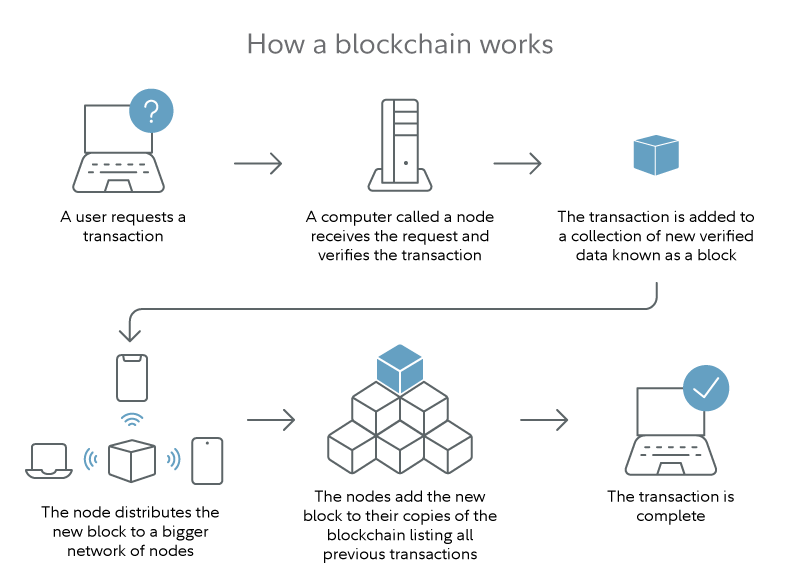
\includegraphics[width=0.8\textwidth]{Figures/block-creation.png}
    \caption{Creación de una transacción y un bloque en una blockchain}
    \label{fig:blockchain-working}
\end{figure}

El proceso de incorporación de una nueva transacción y su respectivo bloque en una blockchain se desarrolla a través de los siguientes pasos:

\begin{enumerate}
    \item Un nodo de la red crea y firma una nueva transacción con su clave privada.
    \item La transacción se propaga a través de la red P2P, donde es recibida por los nodos participantes.
    \item Cada nodo valida la transacción individualmente, verificando la firma del remitente y asegurándose de que este dispone de los fondos o permisos necesarios. Una vez validada, la transacción se añade a un \textit{pool} de transacciones pendientes.
    \item Un nodo (en el caso de PoW, un minero) selecciona un conjunto de transacciones pendientes del \textit{pool} para formar un nuevo bloque. Este bloque incluye las transacciones seleccionadas, el hash del bloque anterior y otros metadatos (como la marca de tiempo y un \textit{nonce} para PoW). El nodo luego calcula el hash de este nuevo bloque y, según el algoritmo de consenso, realiza el trabajo necesario para validarlo. En el caso de PoW, esto implica resolver un problema criptográfico que requiere una cantidad significativa de potencia computacional. En PoS, el nodo debe demostrar que posee una cantidad suficiente de fondos para participar en la validación del bloque.
    \item Una vez que el nodo ha validado el nuevo bloque (o "minado" en PoW), lo difunde a la red. Los demás nodos reciben este bloque y verifican su validez (incluyendo el hash, las transacciones y la prueba de trabajo/participación). Si el bloque es válido, lo añaden a su copia local de la cadena de bloques y descartan las transacciones ya incluidas de su \textit{pool} de pendientes. Si el bloque es inválido, es rechazado por cada nodo y no se añade a la cadena.
\end{enumerate}

De esta forma, la cadena de bloques se actualiza de manera continua y descentralizada, asegurando que todos los nodos de la red mantengan una copia idéntica y consistente del registro de transacciones.

Si bien en su concepción inicial las transacciones en un bloque se asociaban comúnmente a movimientos financieros \cite{satoshi2008bitcoin}, la flexibilidad inherente de la tecnología blockchain permite que los bloques contengan cualquier tipo de información estructurada \cite{bartolomeo2020introduccion}. Esta versatilidad ha sido el motor para el desarrollo de aplicaciones más complejas, destacando entre ellas los \textit{smart contracts} (contratos inteligentes) \cite{sunny2022systematic}.

Los \textit{smart contracts}, o contratos inteligentes, son programas inmutables almacenados en una blockchain que se ejecutan automáticamente al cumplirse condiciones preestablecidas en su código \cite{bulkowska2023implementation}. Su función principal es automatizar procesos en entornos descentralizados, lo que reduce significativamente la dependencia de intermediarios humanos \cite{verma2023overview} y mejora la eficiencia operativa en múltiples sectores \cite{sunny2022systematic}.

Un contrato inteligente se concibe como un conjunto de reglas y lógica de negocio codificadas. Cada contrato posee un código (las reglas) y un estado (la información dinámica) \cite{buterin2013ethereum}. El código es inmutable una vez desplegado en la blockchain mediante una transacción, garantizando la permanencia de las reglas establecidas. Su estado, sin embargo, puede evolucionar a medida que se interactúa con el contrato a través de transacciones. Es importante destacar que, si bien se describen como "auto-ejecutables" por su automatismo al cumplir condiciones, su ejecución es llevada a cabo por los nodos de la red que validan las transacciones e integran los cambios de estado en la cadena \cite{buterin2013ethereum}. Tanto el código como el estado del contrato se almacenan en la blockchain, asegurando su transparencia y disponibilidad pública. Por ejemplo, un contrato inteligente podría gestionar un sistema de votación, donde los participantes envían sus votos y el contrato contabiliza automáticamente los resultados al finalizar el periodo de votación. En la Figura \ref{fig:smart-contract-process} se ilustra el proceso de creación y ejecución de un contrato inteligente, describiendo las etapas desde su definición hasta su implementación y ejecución en la blockchain.

% TODO: use the votation example in this figure to explain the flow of contract creation and execution.
\begin{figure}[!htpb]
    \centering
    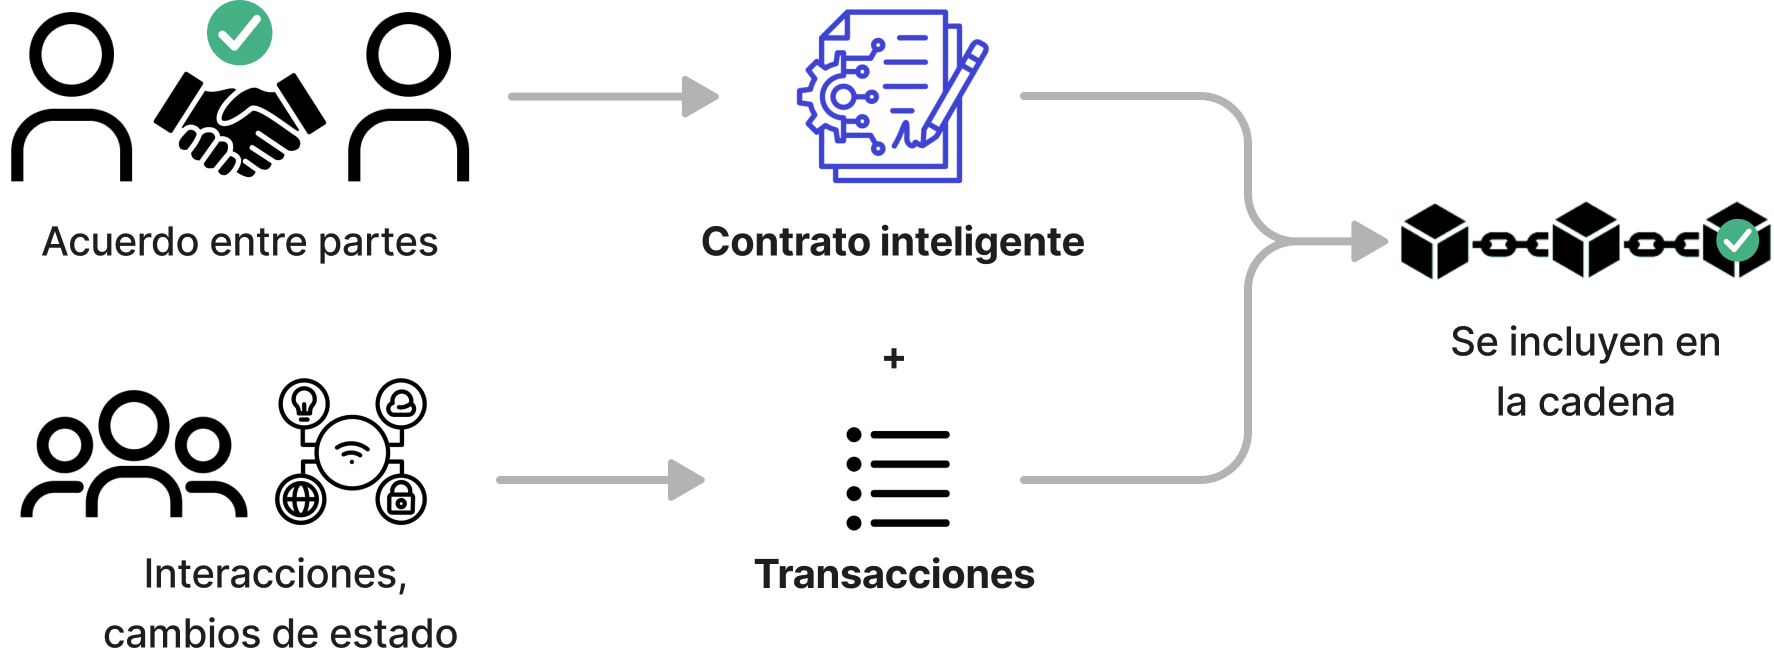
\includegraphics[width=0.8\textwidth]{Figures/smart-contract-process.png}
    \caption{Proceso de creación y ejecución de un contrato inteligente}
    \label{fig:smart-contract-process}
\end{figure}

Para el desarrollo y ejecución de contratos inteligentes, se emplean lenguajes de programación específicos adaptados a cada plataforma blockchain \cite{bartolomeo2020introduccion}. Un ejemplo prominente es \textit{Solidity} \cite{taherdoost2023smart}, utilizado en Ethereum, un lenguaje orientado a objetos diseñado para esta finalidad. Estos contratos pueden interactuar entre sí y con el estado global de la blockchain, habilitando la creación de aplicaciones descentralizadas (dApps) que operan de forma autónoma y sin intermediarios en la red \cite{buterin2013ethereum}.

Sin embargo, los contratos inteligentes enfrentan limitaciones inherentes a las infraestructuras blockchain, principalmente en términos de escalabilidad \cite{kalajdjieski2023databases}. A diferencia de los sistemas centralizados que permiten ejecución paralela y optimización con bases de datos indexadas, los smart contracts operan bajo modelos de ejecución secuencial y replicación completa en cada nodo \cite{taherdoost2023smart}. Esto impacta directamente su rendimiento y complejiza la implementación de algoritmos avanzados. Desde la perspectiva de la ingeniería de software, el desarrollo de contratos inteligentes introduce restricciones no triviales: el código inmutable, los costos asociados al almacenamiento en cadena, la ausencia de llamadas externas directas y los modelos de estado global distribuido. Estas particularidades exigen la adopción de nuevas metodologías y prácticas de diseño seguro, control de flujos y validación estática, muchas de las cuales aún se encuentran en proceso de estandarización \cite{taherdoost2023smart, cepal2021economia}.

En síntesis, los contratos inteligentes constituyen una herramienta computacional que expande las fronteras de la programación distribuida y descentralizada. Si bien su potencial transformador es innegable \cite{taherdoost2023smart}, su desarrollo robusto y seguro representa un desafío activo que abarca múltiples dominios de la computación: desde la teoría de lenguajes formales \cite{hoskinson2017we} y la arquitectura de sistemas distribuidos, hasta la verificación de software, la criptografía aplicada y la integración de datos externos confiables \cite{taherdoost2023smart}.

Debido a la aparición los contratos inteligentes, la tecnología blockchain ha trascendido su origen ligado a las criptomonedas para convertirse en un paradigma disruptivo con aplicaciones transversales en múltiples dominios \cite{bartolomeo2020introduccion, vaigandla2023review}. Se posicionan como un componente fundamental y un impulsor clave de gran parte de las nuevas y complejas soluciones basadas en blockchain, especialmente aquellas que buscan automatizar procesos y gestionar la lógica de negocio directamente en la cadena \cite{sharabati2024blockchain}. Si bien los contratos inteligentes representan una tecnología prometedora, aún se encuentran en una etapa incipiente, lo que implica la existencia de numerosos aspectos por perfeccionar \cite{taherdoost2023smart}. En un contexto más amplio, la tecnología blockchain, incluyendo a los contratos inteligentes, ofrece una serie de ventajas fundamentales y limitaciones inherentes que la distinguen de los sistemas de almacenamiento de datos tradicionales.

% \subsection{Ventajas y Desafíos de Blockchain}

Las características inherentes de la blockchain, detalladas previamente, se traducen en una serie de ventajas que distinguen a blockchain de los sistemas tradicionales. La descentralización propia de su diseño y la consecuente eliminación de intermediarios resultan en una mayor confianza \cite{rejeb2023role} y eficiencia operativa al prescindir de autoridades centrales \cite{sharabati2024blockchain}. La arquitectura basada en registros inmutables garantiza transparencia y trazabilidad completa \cite{sharabati2024blockchain}, permitiendo un historial verificable de cualquier activo o evento, lo cual es crucial para casos de uso como certificación \cite{bartolomeo2020introduccion}, logística \cite{bartolomeo2020introduccion, rejeb2023role} y gestión de residuos \cite{bulkowska2023implementation}. La inmutabilidad de los datos, reforzada por la seguridad criptográfica, asegura la integridad de la información \cite{sunny2022systematic} y una resistencia robusta a manipulaciones maliciosas y puntos únicos de falla \cite{bartolomeo2020introduccion}. Además, la capacidad de automatización de aplicaciones mediante contratos inteligentes optimiza la eficiencia y confiabilidad operativa al ejecutar condiciones lógicas de forma autónoma \cite{bartolomeo2020introduccion}. En conjunto, estas propiedades confieren a blockchain una aplicabilidad transversal que la consolida como una tecnología habilitadora para la transformación digital en sectores diversos como finanzas, salud, IoT, energía, educación y ciudades inteligentes.

Sin embargo, a pesar de sus beneficios, la tecnología blockchain también enfrenta desafíos y limitaciones significativos. Uno de los principales desafíos es la escalabilidad y el rendimiento \cite{tripathi2023comprehensive}. Las blockchains actuales suelen presentar un bajo \textit{throughput} en comparación con los sistemas centralizados \cite{baralla2023waste}, lo cual restringe su aplicación en escenarios de alta frecuencia transaccional. Esto se debe inherentemente a la necesidad de alcanzar un consenso distribuido y a la replicación completa de datos en todos los nodos \cite{tripathi2023comprehensive}. Otro reto importante es la interoperabilidad limitada, que dificulta la integración fluida entre distintas plataformas blockchain con infraestructuras externas preexistentes \cite{tripathi2023comprehensive}. En entornos públicos, la privacidad es una preocupación, ya que, aunque los usuarios pueden operar de forma seudónima, la visibilidad total de las transacciones en la cadena puede comprometer datos sensibles \cite{diez2023web, rennock2018blockchain}. Además, existen vulnerabilidades técnicas inherentes, como el ataque del 51\%, el doble gasto, los ataques Sybil, y la posibilidad de errores en contratos inteligentes mal programados, que requieren atención constante \cite{diez2023web}. La irreversibilidad de las transacciones, si bien es una garantía de seguridad, puede ser problemática ante vulnerabilidades de programación, errores o fraudes, ya que las operaciones registradas no pueden deshacerse \cite{taherdoost2023smart}. Por último, las limitaciones de almacenamiento representan un desafío práctico, dado que los nodos deben almacenar volúmenes crecientes de información, lo cual no escala eficientemente en redes de gran tamaño \cite{taherdoost2023smart}.

Estos desafíos, aunque significativos, están siendo abordados activamente por la investigación y el desarrollo en la comunidad blockchain. La constante evolución de la tecnología y la aparición de nuevas soluciones buscan mitigar estas limitaciones, abriendo el camino para una adopción más amplia \cite{tripathi2023comprehensive, baralla2023waste, taherdoost2023smart}. En este contexto de evolución y superación de barreras, la blockchain ha demostrado su potencial para transformar diversos sectores y abarcar numerosos casos de uso.

% \subsection{Casos de Uso}

En el sector financiero, blockchain ha generado disrupción mediante soluciones para pagos directos (con las llamadas criptomonedas), emisión de bonos, transferencias internacionales y operaciones en mercados de capital \cite{bartolomeo2020introduccion}. Instituciones como Santander y la Bolsa de Comercio de Santiago han adoptado esta tecnología para simplificar transacciones, automatizar registros y eliminar intermediarios \cite{bartolomeo2020introduccion}. Gracias a su estructura descentralizada y sus mecanismos criptográficos, blockchain permite mejorar la trazabilidad de los activos financieros. Pero si bien su uso en finanzas ha sido el más destacado, la tecnología blockchain ha demostrado ser versátil y aplicable a una amplia gama de sectores, cada uno con sus propias necesidades y desafíos.

A nivel gubernamental, blockchain ofrece nuevas herramientas para la modernización del Estado. Permite la gestión segura y verificable de identidades digitales, la trazabilidad de procesos administrativos, y la implementación de sistemas de votación transparentes \cite{vaigandla2023review}. Iniciativas como la European Blockchain Partnership buscan establecer una infraestructura digital pública para servicios intergubernamentales \cite{diez2023web}. Proyectos como QualiChain exploran aplicaciones en el sector público, como la verificación de credenciales profesionales y la gestión automatizada de elegibilidad en concursos públicos \cite{diez2023web}.

En el sector salud, blockchain permite almacenar registros médicos de manera segura y distribuida, mejorando la interoperabilidad entre instituciones, garantizando la integridad de los datos y permitiendo un mayor control por parte de los pacientes \cite{sunny2022systematic, }. También es clave en la trazabilidad de la cadena de suministro farmacéutica y en la supervisión de ensayos clínicos, donde se requiere un alto nivel de confianza y cumplimiento normativo \cite{vaigandla2023review}.

En educación, su aplicación permite la emisión y verificación de certificados académicos inmutables y descentralizados. Universidades como Nicosia o la de Murcia ya utilizan blockchain para certificar diplomas y logros \cite{diez2023web}. Iniciativas como Blockcerts o el pasaporte educativo propuesto por la Unión Europea buscan facilitar la movilidad académica y reducir la falsificación documental. También se exploran aplicaciones como exámenes autoevaluables con contratos inteligentes, recompensas por desempeño y la gestión segura de registros estudiantiles \cite{diez2023web}.

En energía, blockchain permite crear mercados descentralizados para el comercio de energía entre pares, mejora la gestión de certificados de energías renovables, y optimiza la trazabilidad de producción y consumo energético \cite{sunny2022systematic, vaigandla2023review}. Se está utilizando para reducir el impacto ambiental del sector y mejorar la eficiencia operativa de infraestructuras energéticas tradicionales.

En el ámbito de la gestión de la cadena de suministro (SCM), blockchain proporciona una plataforma confiable para garantizar la trazabilidad, autenticidad y visibilidad en tiempo real de productos y materiales \cite{torres2022tendencias, sharabati2024blockchain}. Empresas como IBM, Maersk y FedEx han implementado soluciones blockchain para monitorear inventarios, registrar pagos y reducir disputas logísticas \cite{tripathi2023comprehensive}. Casos como el de Dervinsa en Argentina, que certifica la calidad de productos derivados de residuos de vinificación, y otras iniciativas que aplican trazabilidad a alimentos y textiles, muestran cómo esta tecnología fortalece el control de calidad y la confianza en los mercados \cite{bartolomeo2020introduccion}. Además, en contextos más amplios, blockchain permite una sincronización eficiente entre departamentos, la reducción de riesgos de falsificación y la mejora general de la sostenibilidad operativa \cite{sunny2022systematic}.

En el marco de la economía circular, blockchain se posiciona como un facilitador clave para monitorear ciclos de vida de productos y materiales, ofreciendo transparencia y responsabilidad en la gestión de residuos \cite{bulkowska2023implementation, baralla2023waste}. Diversos tipos de residuos, desde plásticos y vidrio hasta electrónicos y biomédicos, pueden ser gestionados de forma más eficiente mediante el uso de contratos inteligentes que automatizan verificaciones, recompensas e interacciones entre actores de la cadena \cite{baralla2023waste}. Asimismo, se propone la generación de pasaportes digitales de productos y esquemas de incentivos sostenibles, promoviendo hábitos de consumo responsables y nuevos modelos de negocio circulares \cite{baralla2023waste}.

Más allá de estos sectores, blockchain ha demostrado potencial en una variedad de aplicaciones adicionales. En IoT, facilita la recolección y gestión segura de datos en tiempo real \cite{sunny2022systematic}. En contabilidad y auditoría, posibilita libros contables distribuidos con transparencia total y reducción de fraudes \cite{bartolomeo2020introduccion}. También se emplea en caridad y donaciones, trazabilidad inmobiliaria y movilidad inteligente \cite{bartolomeo2020introduccion}. Estos casos de uso evidencian cómo blockchain puede transformar modelos tradicionales mediante estructuras distribuidas, reglas codificadas y registros inmutables. Su implementación efectiva puede contribuir a una mayor eficiencia, confianza y sostenibilidad en múltiples áreas críticas del desarrollo económico, social y tecnológico.

Si bien las aplicaciones de blockchain se extienden a numerosos sectores, uno de los ámbitos donde esta tecnología adquiere un protagonismo creciente es en la economía circular. La necesidad de trazar el flujo de materiales, certificar la autenticidad de los procesos productivos y garantizar la transparencia en la gestión de residuos ha posicionado a blockchain como una herramienta protagónica para habilitar modelos circulares sostenibles. En particular, su capacidad para registrar datos inmutables y automatizar interacciones mediante contratos inteligentes permite estructurar sistemas de trazabilidad que no sólo mejoran la eficiencia, sino que también fortalecen la confianza entre actores y fomentan la rendición de cuentas \cite{sharabati2024blockchain, rejeb2023role}. A continuación, se analiza con mayor profundidad el rol de blockchain en el diseño e implementación de estrategias de economía circular, con énfasis en sus aplicaciones concretas en trazabilidad de materiales en la cadena de suministros y gestión de residuos.

\section{Economía circular}

La economía circular se presenta como una evolución del modelo económico lineal que ha prevalecido desde la Revolución Industrial. Mientras el enfoque lineal se basa en una secuencia unidireccional de extracción, producción, consumo y descarte, la economía circular propone un rediseño profundo de este paradigma al introducir principios de regeneración, reutilización y cierre de ciclos. Su objetivo es maximizar el valor de los recursos materiales y energéticos a lo largo del tiempo, minimizando al mismo tiempo el impacto ambiental y la dependencia de recursos no renovables.

El modelo lineal ha demostrado ser altamente efectivo para fomentar el crecimiento económico, pero también ha generado efectos colaterales significativos que lo hacen insostenible en el largo plazo. Entre los principales problemas que motivan la transición hacia un enfoque circular se encuentran el agotamiento progresivo de los recursos naturales, la acumulación masiva de residuos y la insostenibilidad de los patrones de consumo. La extracción intensiva de materias primas, muchas veces por encima de su tasa de regeneración, ha provocado deforestación, pérdida de biodiversidad y una creciente presión sobre ecosistemas frágiles. Al mismo tiempo, el diseño de productos con ciclos de vida cortos —como ocurre con la moda rápida o los dispositivos electrónicos desechables— genera residuos prematuros y desaprovecha el valor residual de los materiales. % Esta dinámica es agravada por el aumento previsto en los costos de las materias primas y la energía, lo que cuestiona la viabilidad económica del modelo lineal en contextos futuros.

Frente a estos desafíos, la economía circular emerge como un modelo restaurativo y regenerativo por diseño. Promueve prácticas como la reutilización, la reparación, el reciclaje de alta calidad y la remanufactura, con el propósito de mantener los productos y materiales en uso durante el mayor tiempo posible. Se basa en tres principios fundamentales: eliminar residuos y contaminación desde el diseño, mantener los recursos en uso mediante bucles cerrados, y regenerar sistemas naturales en lugar de degradarlos. En lugar de centrarse únicamente en reducir impactos negativos, busca generar valor positivo para la economía, la sociedad y el medio ambiente.

La economía circular ofrece una serie de ventajas frente al modelo lineal. Desde el punto de vista económico, puede fomentar nuevos modelos de negocio, reducir costos operativos y mejorar la eficiencia en el uso de materiales y energía. Además, contribuye a la creación de empleo, disminuye la dependencia de materias primas importadas y mejora la resiliencia económica. Ambientalmente, permite reducir emisiones de gases de efecto invernadero, minimizar la generación de residuos y preservar ecosistemas. A nivel social, promueve una cultura de consumo responsable, empodera a los ciudadanos y mejora la equidad mediante la formalización de sectores informales como el reciclaje.

Sin embargo, también enfrenta barreras significativas. Existen desafíos culturales, normativos y tecnológicos que dificultan su implementación a gran escala. La transición requiere una transformación estructural en los sistemas productivos, inversión en infraestructura, marcos regulatorios adecuados y políticas de incentivos claros. Asimismo, implica repensar la educación y la formación de trabajadores para adaptarse a nuevas dinámicas laborales. En muchos contextos, como América Latina y el Caribe, también se identifican limitaciones institucionales y de gobernanza que deben ser abordadas para permitir una adopción efectiva del modelo.

En definitiva, la economía circular no debe entenderse como una simple mejora del modelo actual, sino como una evolución hacia un sistema más integrado, resiliente y sostenible. Su implementación exige un enfoque sistémico, colaboración multisectorial y el uso estratégico de tecnologías habilitadoras como la trazabilidad digital y blockchain.

% TODO improve this connection between the two sections

Para comprender en profundidad la diferencia estructural entre la economía lineal y la economía circular, se incluyen a continuación esquemas comparativos que ilustran el flujo de recursos en ambos modelos. En el enfoque lineal, la cadena de suministro se organiza como un proceso unidireccional: los recursos son extraídos, transformados en productos, consumidos y finalmente desechados. Este modelo ignora el valor residual de los materiales, genera una creciente acumulación de residuos y no contempla mecanismos para reincorporar los productos al ciclo productivo una vez finalizada su vida útil.

En contraste, la economía circular redefine el papel de la cadena de suministro transformándola en una red cerrada y regenerativa. El objetivo es mantener los productos, componentes y materiales en uso el mayor tiempo posible mediante estrategias de reutilización, reparación, remanufactura y reciclaje. La cadena se vuelve más dinámica e interdependiente, integrando bucles de retroalimentación entre los diferentes actores de la cadena de valor, incluyendo consumidores, productores, proveedores y gestores de residuos. Esta visión implica una transformación profunda del diseño de productos, los procesos logísticos, la distribución y la gestión del fin de vida.

Para llevar a cabo esta transición sistémica desde un modelo lineal hacia uno circular, se requieren cambios estructurales en múltiples niveles. Entre los habilitadores clave de este proceso se encuentra la trazabilidad, entendida como la capacidad de rastrear el origen, el uso y el destino de materiales y productos a lo largo de toda su vida útil. La trazabilidad permite verificar compromisos ambientales, controlar impactos, optimizar la logística inversa y empoderar tanto a consumidores como a instituciones para adoptar decisiones basadas en información confiable. Su implementación resulta esencial para garantizar la transparencia, la confianza entre actores y la eficiencia en los flujos circulares.

Es importante destacar que esta transición ya se encuentra en marcha. Diversos países, regiones y sectores productivos han comenzado a incorporar principios circulares en sus estrategias de desarrollo, en muchos casos impulsados por marcos regulatorios, acuerdos internacionales y metas vinculadas a la sostenibilidad ambiental. En este contexto, las políticas públicas han asumido un rol central como motores de adopción, ofreciendo instrumentos normativos, fiscales y de gobernanza que facilitan la transformación del sistema económico. A continuación, se analizarán estas políticas sustentables como eje estratégico para avanzar hacia una economía más circular y resiliente.

\subsection{Políticas sustentables}

En el proceso de transición hacia modelos de desarrollo más sostenibles, la Unión Europea ha asumido un rol pionero en la implementación de políticas públicas alineadas con la economía circular. Iniciativas como el Pacto Verde Europeo, la Ley Europea del Clima o los marcos regulatorios vinculados al paquete Objetivo 55 han consolidado a Europa como un referente global en materia de sustentabilidad ambiental. Estas políticas no solo promueven la descarbonización de la economía, sino que también introducen principios de circularidad en sectores como la industria, la energía, la movilidad y la gestión de residuos, reconfigurando las cadenas de suministro hacia sistemas más regenerativos, transparentes y trazables.

Sin embargo, el mayor hito internacional en la construcción de una visión compartida sobre sustentabilidad ha sido, sin duda, la adopción de los Objetivos de Desarrollo Sostenible (ODS) de Naciones Unidas en 2015. Este conjunto de 17 objetivos interconectados, acompañados por 169 metas y más de 230 indicadores, propone una agenda universal que orienta las políticas públicas hacia un desarrollo económico, social y ambiental equilibrado para 2030.

% \begin{figure}[!htpb]
% 		\centering
% 		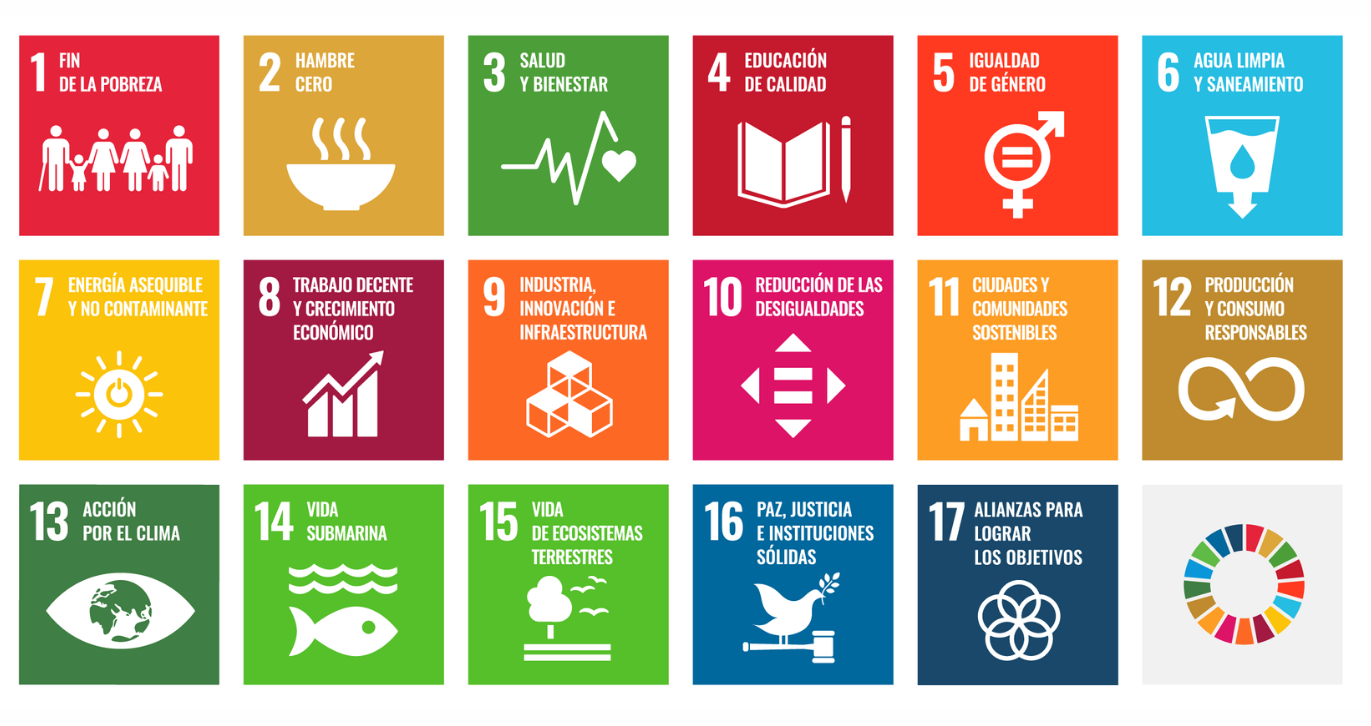
\includegraphics[width=0.8\textwidth]{figures/ods.png}
% 		\caption{Objetivos de Desarrollo Sostenible (ODS) de Naciones Unidas.}
% 		\label{fig:ods}

El objetivo general de los ODS es erradicar la pobreza, proteger el planeta y garantizar la paz y prosperidad para todas las personas. En relación con la economía circular, existen cinco objetivos particularmente relevantes que guían tanto los marcos normativos como las estrategias de innovación en producción, consumo y gestión de residuos:

\begin{itemize}
\item \textbf{ODS 7: Energía asequible y no contaminante.} Promueve el acceso universal a fuentes de energía limpias, eficientes y modernas, fundamentales para la transición a una economía circular descarbonizada.
\item \textbf{ODS 11: Ciudades y comunidades sostenibles.} Plantea la necesidad de gestionar de manera integrada los recursos urbanos, incluyendo residuos, infraestructura y movilidad, en articulación con una trazabilidad eficiente de los flujos materiales.
\item \textbf{ODS 12: Producción y consumo responsables.} Es el núcleo del paradigma circular, impulsando el diseño sostenible de productos, el uso eficiente de recursos, la minimización de residuos y la promoción de modelos de cadena de suministro regenerativos.
\item \textbf{ODS 13: Acción por el clima.} Vincula la circularidad con la reducción de emisiones y la adaptación al cambio climático, incentivando políticas que rediseñen los sistemas productivos de alto impacto ambiental.
\item \textbf{ODS 15: Vida de ecosistemas terrestres.} Apunta a la restauración y conservación de ecosistemas degradados, objetivos que sólo pueden alcanzarse mediante modelos productivos basados en ciclos cerrados de materia y energía.
\end{itemize}

Los ODS han generado un marco de referencia común que ha influido fuertemente en las agendas de sostenibilidad a nivel global, incluyendo América Latina. Aunque en la región la adopción de políticas circulares aún es incipiente en comparación con Europa, se observan avances significativos. Por ejemplo, varios países han comenzado a incorporar la responsabilidad extendida del productor, prohibiciones de plásticos de un solo uso y normativas orientadas a la reutilización y reciclado de materiales. Estas políticas buscan reestructurar las cadenas de valor y fomentar prácticas productivas y logísticas compatibles con los principios de circularidad.

En Argentina, la Estrategia Nacional de Consumo y Producción Sostenibles se destaca como el instrumento central para avanzar hacia la economía circular. Este plan integra medidas normativas, educativas, tecnológicas y financieras, orientadas a fortalecer la sostenibilidad en toda la cadena de producción y consumo. Se promueve activamente el uso de tecnologías limpias, la gestión sostenible de recursos, y la incorporación de criterios ambientales en compras públicas, reconociendo el rol de la trazabilidad como mecanismo para garantizar la transparencia, eficiencia y cumplimiento normativo en los procesos productivos.

Si bien estos esfuerzos representan un paso importante, los desafíos estructurales persisten. La región enfrenta obstáculos en términos de infraestructura, financiamiento, coordinación institucional y disponibilidad de información confiable. A pesar de ello, el impulso dado por los ODS ha generado una convergencia regional que permite imaginar una transición hacia modelos circulares, sostenida por políticas públicas que consideran no sólo las metas globales, sino también las realidades locales.

En este escenario, la transformación hacia una economía circular no puede pensarse sin una reconfiguración profunda de las cadenas de suministro, que constituyen la columna vertebral de los sistemas productivos. La implementación de políticas sustentables, tanto en Europa como en América Latina, ha puesto en evidencia la necesidad de contar con mecanismos que permitan monitorear, verificar y optimizar el flujo de materiales a lo largo de todo el ciclo de vida de los productos. En este sentido, la trazabilidad emerge como una herramienta clave para operacionalizar los principios de la circularidad, asegurando la transparencia, la calidad y la responsabilidad en cada etapa del proceso. La siguiente sección abordará con mayor detalle cómo se articula esta relación entre cadenas de suministro y trazabilidad, y cuál es su rol estratégico en la transición hacia modelos económicos más sostenibles, resilientes y regenerativos.

\subsection{Cadena de suministro}

La cadena de suministro constituye el entramado logístico, operativo y estratégico que permite el flujo de materiales, información y recursos desde la extracción de materias primas hasta la llegada del producto al consumidor final. Este sistema complejo, que involucra a múltiples actores —proveedores, fabricantes, distribuidores, minoristas, consumidores y, en algunos casos, gestores de residuos y autoridades regulatorias—, busca garantizar que los bienes y servicios se produzcan y entreguen de manera eficiente, segura y rentable. En su concepción tradicional, la cadena de suministro ha estado orientada a la eficiencia lineal, es decir, maximizar el rendimiento del flujo "de origen a destino", sin considerar el impacto postconsumo o el valor residual de los materiales.

Sin embargo, en el contexto de la economía circular, la cadena de suministro asume una nueva lógica de funcionamiento. En lugar de ser una secuencia finita de pasos que culminan con la disposición del producto, se transforma en un sistema regenerativo y cíclico, en el cual los materiales son diseñados para permanecer en uso el mayor tiempo posible, ser reutilizados, reacondicionados o reciclados. Esta visión circular implica rediseñar productos, procesos y relaciones para mantener el valor de los recursos a lo largo del tiempo, evitando su descarte prematuro y reduciendo la necesidad de materias primas vírgenes.

Esta transformación se estructura en una serie de etapas conectadas, que conforman el nuevo ciclo productivo circular: producción, consumo, recolección de residuos, transporte, clasificación y disposición, y finalmente, reciclaje o reacondicionamiento. Cada una de estas etapas requiere coordinación, trazabilidad e integración de datos, especialmente en sistemas donde intervienen múltiples organizaciones y tecnologías. 

La trazabilidad —entendida como la capacidad de rastrear un producto desde su origen hasta su destino y más allá— se vuelve un habilitador fundamental que conecta todas las fases del proceso, asegurando integridad, transparencia y responsabilidad en cada paso.

% TODO: check this connection with the previous section

La trazabilidad es la capacidad de seguir el recorrido completo de un producto, material o componente a lo largo de toda la cadena de suministro, desde su origen hasta su destino final, e incluso más allá, en escenarios de reutilización o reciclaje. Su objetivo principal es reconstruir el historial de producción, transformación y movimiento de un bien, permitiendo conocer su composición, ubicación, responsables y condiciones de manejo en cada etapa del proceso. Esta información resulta clave no solo para verificar la autenticidad del producto, sino también para asegurar estándares de calidad, cumplimiento normativo, eficiencia operativa y sostenibilidad ambiental.

En el contexto de la cadena de suministro, la trazabilidad se aplica de forma transversal, es decir, atraviesa e interconecta todas las fases del ciclo: desde el diseño y la fabricación, hasta la distribución, el consumo, la gestión de residuos y el reciclaje. No se trata de una función aislada, sino de una infraestructura digital que permite registrar, verificar y compartir información crítica entre todos los actores del sistema. De este modo, la trazabilidad facilita la coordinación entre partes, reduce los riesgos asociados a errores, fraudes o contaminaciones, y mejora la capacidad de respuesta ante incidentes o fallas en la cadena.

No obstante, su implementación conlleva desafíos importantes. Las cadenas de suministro tradicionales suelen estar fragmentadas y utilizar sistemas de información heterogéneos o poco interoperables. Muchos registros todavía se realizan en papel o en bases de datos centralizadas, lo que aumenta la vulnerabilidad frente a errores humanos, pérdidas de datos o manipulaciones. Además, la ausencia de estándares unificados y la reticencia a compartir datos entre organizaciones limitan la visibilidad total del flujo de productos y materiales.

Los sistemas tradicionales de trazabilidad a menudo dependen de terceros de confianza, con datos almacenados en papel o en bases de datos centralizadas. Estos enfoques son propensos a problemas de integridad de datos, altos costos, ineficiencias por procesos manuales, errores humanos y manipulación. En contraste, Blockchain ofrece un nuevo modelo donde la autenticidad no es verificada por un tercero, sino por la propia red de nodos mediante consenso. La naturaleza descentralizada de Blockchain, donde cada participante tiene una copia del registro, contrasta con el modelo centralizado, donde un error puede llevar a la pérdida de información o comprometer su integridad.

Para abordar estos desafíos, se ha desarrollado un conjunto de tecnologías que fortalecen los sistemas de trazabilidad. Entre las más utilizadas se encuentran los códigos de barras y las etiquetas RFID, que permiten la identificación automática de productos; los sensores IoT, que capturan datos en tiempo real sobre condiciones ambientales o de transporte; los sistemas ERP y de gestión logística, que centralizan y organizan la información operativa; y, más recientemente, la tecnología blockchain, que introduce una capa adicional de seguridad, inmutabilidad y transparencia.

Blockchain, en particular, permite registrar cada transacción o evento de la cadena en un registro digital descentralizado e inalterable. Esto garantiza que todos los actores tengan acceso a un historial común y verificable, eliminando la necesidad de intermediarios o auditores externos. Combinando contratos inteligentes y plataformas de análisis de datos, la trazabilidad basada en blockchain permite no solo conocer lo que ocurrió, sino también automatizar respuestas ante condiciones predefinidas, reduciendo los tiempos de reacción y aumentando la confianza entre las partes.

En la cadena de suministro (SCM), Blockchain desempeña un papel transformador. Aporta un aumento significativo en la seguridad, confidencialidad, trazabilidad, transparencia, precisión de datos, privacidad, eficiencia, responsabilidad y confianza. Se utiliza en diversos sectores como la agricultura, alimentos, industria, marítimo y medioambiental. Por ejemplo, en el sector alimenticio, impulsa el valor percibido del producto y la calidad, además de fortalecer la confianza entre las partes interesadas. Para el sector industrial, se enfoca en la planeación y el intercambio de información para una mayor sostenibilidad. En el sector textil, mejora los procesos internos, la trazabilidad y previene la falsificación. La tecnología Blockchain, unida a IoT, puede proporcionar soluciones eficientes y eficaces para la cadena de suministro, mejorando la recopilación de datos y los beneficios para las partes interesadas. Si bien su aplicación aún está en desarrollo, su potencial para optimizar la trazabilidad y la sostenibilidad en la gestión de residuos es ampliamente reconocido.

La trazabilidad, por lo tanto, se convierte en un habilitador clave para la transición hacia modelos de economía circular. Permite no solo verificar el cumplimiento de estándares ambientales y sociales, sino también optimizar el uso de recursos, reducir desperdicios y fomentar la reutilización y el reciclaje. En un contexto donde la sostenibilidad es cada vez más prioritaria, contar con sistemas de trazabilidad robustos y confiables resulta esencial para garantizar la transparencia, la eficiencia y la responsabilidad en las cadenas de suministro.

\subsection{Proceso de producción y reciclaje en la economía circular}

En el marco de la economía circular, los procesos de producción y reciclaje dejan de concebirse como etapas aisladas y unidireccionales para integrarse en un sistema dinámico y regenerativo. Este sistema busca maximizar el valor de los materiales a lo largo del tiempo, manteniéndolos en uso durante el mayor tiempo posible, y reintroduciéndolos en el ciclo económico una vez finalizada su vida útil. A diferencia del modelo lineal, donde los productos son descartados tras el consumo, la economía circular plantea un circuito continuo que requiere rediseñar tanto las formas de producir como las estrategias de recuperación.

El proceso de producción comienza en la etapa de diseño, donde se decide la composición de los productos considerando criterios de ecoeficiencia, reutilización y reciclabilidad. Aquí intervienen diseñadores, ingenieros y proveedores de materias primas, quienes priorizan materiales reciclados o de bajo impacto ambiental. A continuación, durante la fabricación, los procesos industriales buscan reducir el uso de recursos y minimizar las emisiones, integrando tecnologías limpias y eficientes. En esta fase, los productos terminados o semielaborados quedan registrados con información detallada sobre su origen, composición y trazabilidad, lo cual permite una futura gestión más eficiente de su reciclaje.

Una vez que los productos son utilizados por los consumidores, comienza el ciclo inverso de valorización. Cuando estos artículos llegan al fin de su vida útil, se convierten en residuos que deben ser recolectados, transportados, clasificados y reacondicionados. Este proceso de reciclaje involucra a recolectores, centros de acopio, plantas de tratamiento, recicladores industriales y fabricantes secundarios. Durante la recolección, tecnologías como sensores IoT, lectores de códigos QR o etiquetas RFID permiten registrar información sobre la identidad del recolector, la cantidad, el tipo y las condiciones del residuo. Esta información permite monitorear flujos y brindar transparencia en la cadena.

Posteriormente, los residuos son transportados a instalaciones donde se clasifican y segregan según su tipo y calidad. Este paso es fundamental para evitar contaminaciones cruzadas y asegurar un reciclaje efectivo. Finalmente, los materiales seleccionados se someten a procesos de reciclaje o reacondicionamiento, reincorporándolos al sistema productivo como insumos o productos reutilizables. Aquí, tecnologías como blockchain pueden documentar cada transacción o transformación, fortaleciendo la integridad del proceso y fomentando la confianza entre los actores.

Existen diversos materiales reciclables, cada uno con características particulares. El papel y cartón son ampliamente reciclados y fáciles de recolectar, mientras que los metales —como el aluminio, el acero o el cobre— conservan sus propiedades tras múltiples ciclos. Los residuos electrónicos (RAEE) presentan un alto valor por su contenido en metales preciosos, aunque requieren procesos especializados. Los plásticos, si bien representan un desafío por su heterogeneidad, pueden reciclarse eficientemente si se rediseñan los envases y se simplifican sus composiciones. Los residuos orgánicos son compostables o pueden aprovecharse energéticamente. Finalmente, el vidrio destaca como el material circular por excelencia: puede reciclarse infinitas veces sin perder calidad, su estructura es químicamente estable, y su reciclaje requiere menos energía que su producción original. Estas cualidades lo convierten en un insumo ideal para sistemas de economía circular bien diseñados.

El siguiente esquema conceptual sintetiza estas etapas como un ciclo cerrado, donde cada fase se conecta mediante mecanismos de trazabilidad digital que permiten el seguimiento de los materiales desde su origen hasta su reincorporación al sistema:

% \begin{figure}[!htpb]
%     \centering
%     % \includegraphics[width=\textwidth]{ruta/a/diagrama_produccion_reciclaje.png}
%     \fbox{\parbox{0.9\textwidth}{\centering \textit{Placeholder: diagrama del proceso de producción y reciclaje con trazabilidad circular}}}
%     \caption{Ciclo circular de producción y reciclaje con trazabilidad}
% \end{figure}

Este enfoque refleja cómo el diseño de productos, la gestión eficiente de los residuos y la integración de tecnologías como blockchain pueden transformar las cadenas de suministro tradicionales en sistemas circulares, resilientes y sostenibles.

\subsection{Cadena de suministro del vidrio}

El vidrio es uno de los materiales más representativos de la economía circular por su capacidad única de ser reciclado indefinidamente sin perder calidad. Esta propiedad lo convierte en un recurso estratégico para reducir la demanda de materias primas vírgenes, minimizar residuos y disminuir la huella de carbono asociada a la producción industrial. A diferencia de otros materiales cuyo reciclaje implica degradación, el vidrio conserva íntegramente sus características físicas y químicas, permitiendo su reintegración al ciclo productivo tantas veces como sea necesario.

La cadena de suministro del vidrio en un modelo circular abarca múltiples etapas interconectadas, desde la extracción de materias primas hasta la reincorporación del material reciclado a nuevos ciclos de producción. El proceso comienza con el diseño del producto, etapa clave para asegurar su durabilidad, reutilización y posterior reciclabilidad. Le sigue la producción industrial, donde se funden arena, sosa y caliza a altas temperaturas, frecuentemente combinadas con calcín (vidrio reciclado triturado) para reducir el consumo energético. Luego, los envases fabricados son distribuidos y utilizados por los consumidores, quienes pueden reutilizarlos o, una vez descartados, ingresarlos a circuitos de reciclaje. La recolección diferenciada, el transporte, la clasificación y limpieza del material son esenciales para garantizar un reciclaje de calidad. Finalmente, el vidrio tratado se funde nuevamente y se convierte en materia prima secundaria para nuevos envases, cerrando así el ciclo.

Este sistema se representa esquemáticamente en el siguiente diagrama, que ilustra las etapas circulares desde el diseño hasta la refabricación y reincorporación al ciclo productivo:

% \begin{figure}[!htpb]
%     \centering
%     % \includegraphics[width=\textwidth]{ruta/a/diagrama_cadena_vidrio.png}
%     \fbox{\parbox{0.9\textwidth}{\centering \textit{Placeholder: diagrama de la cadena circular de suministro y reciclaje del vidrio}}}
%     \caption{Cadena circular de suministro y reciclaje del vidrio}
% \end{figure}

En Mendoza, la cadena del vidrio adquiere una importancia estratégica por su estrecha vinculación con la industria vitivinícola, uno de los principales motores económicos de la región. La provincia cuenta con una única empresa que produce y recicla envases de vidrio a escala industrial: Verallia. Esta compañía internacional cubre la totalidad de la demanda local de botellas y frascos, fabricando envases para vinos, espumantes, cervezas, licores y alimentos. El proceso de producción en Verallia incluye desde la selección y mezcla de materias primas hasta la formación, inspección y distribución de los envases, con la integración progresiva de vidrio reciclado como parte del insumo.

Verallia ha reconocido públicamente que la mayor dificultad de su industria es la elevada emisión de dióxido de carbono, por lo que ha adoptado una estrategia dual orientada a optimizar el reciclaje y fomentar la reutilización del vidrio. Bajo esta lógica, ha desarrollado el programa “Vidrio, una acción transparente” en alianza con el Gobierno de Mendoza, mediante el cual se promueve la recolección de envases descartados, destinando los ingresos generados al apoyo de organizaciones benéficas. Esta iniciativa, aunque aún incipiente, representa un esfuerzo por avanzar hacia una cadena de suministro más circular y socialmente responsable.

Sin embargo, el reciclaje de vidrio en Mendoza enfrenta desafíos estructurales. La tasa de recuperación aún es baja, las métricas oficiales son escasas y las políticas de incentivo son limitadas. La logística de recolección depende en gran medida de la voluntad ciudadana y carece de sistemas obligatorios o premiantes que aseguren su masividad. En este contexto, el rol de actores industriales como Verallia resulta central para impulsar transformaciones sostenibles en la cadena del vidrio, tanto mediante la innovación tecnológica como a través de la articulación público-privada.

Más allá del caso mendocino, el vidrio sigue siendo uno de los materiales más valiosos dentro de una economía circular bien implementada. Su durabilidad, estabilidad química, transparencia y capacidad de reciclaje total lo convierten en un insumo ideal para cerrar ciclos productivos sin pérdidas de calidad ni de valor. Avanzar hacia una cadena del vidrio plenamente circular requiere optimizar cada etapa, desde el diseño y la fabricación hasta la trazabilidad del reciclaje, consolidando sistemas logísticos eficientes, ciudadanos comprometidos y políticas públicas robustas que garanticen su sostenibilidad a largo plazo.

\section{Proyectos y trabajos relacionados}

% TODO: fill this section with related projects and works

\begin{block}[todo]
    \textit{Fill this section with related projects and works}
\end{block}

[Mencionar y describir de manera fluída algunos de todos estos proyectos, comenzando desde lo más simple a lo más complejo. Primero tecnología para incentivar reciclaje, luego uso de blockchain en cadena de suministros, luego específicamente orientado a sustentabilidad y por último que además se concentren en dar trazabilidad. Sacar en limpio los aportes relevantes de cada uno y los puntos débiles (que resolverá mi trabajo)].

Tecnología con incentivos para el reciclaje:
\begin{itemize}
    \item DRS (PFAND, Alemania)
    \item Reciclos (España)
    \item Colmena (Argentina)
    \item Greenly Points (Argentina)
    \item Plastic Bank (Canadá)
\end{itemize}

Aplicaciones de tecnología blockchain en la cadena de suministro para logística/trazabilidad:
\begin{itemize}
    \item Signeblock (España)
\end{itemize}

Uso de tecnología blockchain en la cadena de suministro para la sustentabilidad:
\begin{itemize}
    \item Modelo para la gestión de residuos [baralla2023waste]
    \item Modelo ZERO para el Reciclaje de Plásticos con Tecnología Blockchain
    \item Uso de Blockchain y Marcadores Moleculares para el Manejo Sostenible de Residuos Plásticos
\end{itemize}

Uso de tecnología blockchain en la cadena de suministro para trazabilidad para Sustentabilidad:
\begin{itemize}
    \item Circularise (Holanda)
    \item Circulor (Reino Unido)
\end{itemize}

[Debo cerrar de alguna manera con conclusión o un párrafo el marco teórico antes de saltar a metodología? Quizás contar dónde acotamos el problema vistos los proyectos preexistentes? Dónde cuento que elegimos vidrio en Mendoza por el vino y que vamos a hacer un sistema de trazabilidad específicamente para esa cadena de suministros y todos sus actores??]
